\documentclass{article}

\usepackage{color,amsmath,amssymb,graphicx,fancyhdr,amsfonts,amsthm,algorithmic,verbatim,bbold,environ}
\usepackage{algorithm,hyperref}
\usepackage{mkolar_definitions}
\usepackage{multirow}
\usepackage{diagbox}
\usepackage{longtable,booktabs}
\usepackage[left=2cm,top=2cm,right=2cm]{geometry}
\numberwithin{algorithm}{section}

\newcommand{\tightlist}{%
  \setlength{\itemsep}{0pt}\setlength{\parskip}{0pt}}


%%%%%%%%%%%%%%%%%%%%%%%%%%%%%
\newcommand{\tta}{\theta}
\newcommand{\lag}{\left\langle}
\newcommand{\rag}{\right\rangle}
\newcommand{\lnorm}{\left\|}
\newcommand{\rnorm}{\right\|}
%%%%%%%%%%%%%%%%%%%%%%%%%%%%%



\title{CS258 Information Theory Homework 6}
\author{Zhou Litao 518030910407 F1803016}
\date{\today}
\begin{document}
\maketitle

%%%%%%%%%%%%%%%%%%%%%%%%%%%%%%%%%%%%%%%%%%
%%%%%%%%%%%%%                 %%%%%%%%%%%%
%%%%%%%%%%%%%    EXERCISE 1   %%%%%%%%%%%%
%%%%%%%%%%%%%                 %%%%%%%%%%%%
%%%%%%%%%%%%%%%%%%%%%%%%%%%%%%%%%%%%%%%%%%
\begin{exercise}[BSC]{Calculate the channel capacity of BSC.
  \begin{figure}[H]
    \centering
    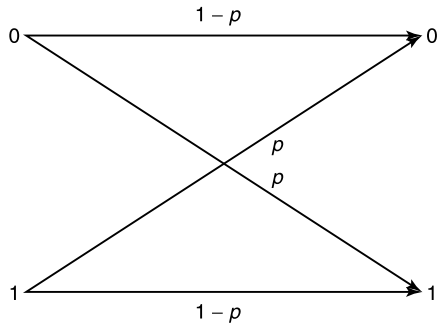
\includegraphics[height=3cm]{img/6-1.png}
    \caption{Binary Symmetric Channel}
    \label{fig:bsc}
  \end{figure}}
  \begin{solution}
  \begin{equation}\begin{aligned}
    C &=\max_{p(x)} I(X ; Y) \\
    &=\max_{p(x)} (H(Y)-H(Y | X) )\\
    &=\max_{p(x)} (H(Y)-\sum p(x) H(Y | X=x) )\\
    &=\max_{p(x)} (H(Y)-\sum p(x) H(p)) \\
    &=\max_{p(x)} (H(Y) - H(p)) = \log 2 - H(p)
    \end{aligned}\end{equation}
  The maximal value can be obtained when $X$ and $Y$ are uniformly distributed.
  \end{solution}
  \label{ex1}
\end{exercise}

%%%%%%%%%%%%%%%%%%%%%%%%%%%%%%%%%%%%%%%%%%
%%%%%%%%%%%%%                 %%%%%%%%%%%%
%%%%%%%%%%%%%    EXERCISE 2   %%%%%%%%%%%%
%%%%%%%%%%%%%                 %%%%%%%%%%%%
%%%%%%%%%%%%%%%%%%%%%%%%%%%%%%%%%%%%%%%%%%
\begin{exercise}[BSC]{Calculate the channel capacity of BEC.
  \begin{figure}[H]
    \centering
    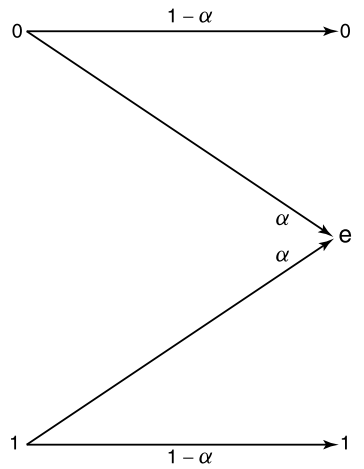
\includegraphics[height=4cm]{img/6-2.png}
    \caption{Binary Erasure Channel}
    \label{fig:bec}
  \end{figure}}
  \begin{solution}
    \begin{equation}\begin{aligned}
      C &=\max _{p(x)} I(X ; Y) \\
      &=\max _{p(x)}(H(Y)-H(Y | X))\\
      &=\max _{p(x)} (H(Y)-H(\alpha))
      \end{aligned}\end{equation}
      Let $\Pr\left(X = 1\right) = \pi$, then
      \begin{equation}
        \begin{aligned}
          H(Y) &= H((1-\pi)(1-\alpha),\alpha,\pi(1-\alpha)) \\
          &= H(\alpha) + (1-\alpha)H(\pi) \\
          C &= \max_{p(x)} (H(Y)-H(\alpha)) \\
          &= \max_{\pi} ((1-\alpha)H(\pi)+H(\alpha)-H(\alpha)) \\
          &= \max_{\pi} (1-\alpha)H(\pi) = 1-\alpha
        \end{aligned}
      \end{equation}
      The maximal value can be obtained when $X$ is uniformly distributed.
  \end{solution}
  \label{ex2}
\end{exercise}

%%%%%%%%%%%%%%%%%%%%%%%%%%%%%%%%%%%%%%%%%%
%%%%%%%%%%%%%                 %%%%%%%%%%%%
%%%%%%%%%%%%%    EXERCISE 3   %%%%%%%%%%%%
%%%%%%%%%%%%%                 %%%%%%%%%%%%
%%%%%%%%%%%%%%%%%%%%%%%%%%%%%%%%%%%%%%%%%%
\begin{exercise}[Using two channels at once]{Consider two discrete memoryless channels $\left(\mathcal{X}_{1}, p\left(y_{1} | x_{1}\right), \mathcal{Y}_{1}\right)$ and $\left(\mathcal{X}_{2}, \right.$  $\left. p\left(y_{2} | x_{2}\right), \mathcal{Y}_{2}\right)$ with capacities $C_{1}$ and $C_{2}$ respectively. A new channel $\left(\mathcal{X}_{1} \times \mathcal{X}_{2}, p\left(y_{1} | x_{1}\right) \times p\left(y_{2} | x_{2}\right), \mathcal{Y}_{1} \times \mathcal{Y}_{2}\right)$ is formed in which $x_{1} \in \mathcal{X}_{1}$ and $x_{2} \in \mathcal{X}_{2}$ are sent simultaneously, resulting in $\mathcal{Y}_{1}, \mathcal{Y}_{2} .$ Find the capacity of this channel.}
  \begin{solution} By condition we know that $p(y_1,y_2|x_1,x_2) = p\left(y_{1} | x_{1}\right) \times p\left(y_{2} | x_{2}\right)$. It follows by definition that 
    \begin{equation}
      H(Y_1,Y_2|X_1,X_2) = H(Y_1|X_1)+H(Y_2|X_2).
    \end{equation}
    Therefore, 
    \begin{equation}
      \begin{aligned}
        I(X_1,X_2;Y_1,Y_2) &= H(Y_1,Y_2) - H(Y_1,Y_2|X_1,X_2) \\
        &= H(Y_1,Y_2) - H(Y_1|X_1) - H(Y_2|X_2) \\
        &\le H(Y_1) + H(Y_2) - H(Y_1|X_1) - H(Y_2|X_2) \\
        &= I(Y_1;X_1) + I(Y_2;X_2) \\
        &\le C_1 + C_2
      \end{aligned}
    \end{equation}
    Hence $C = C_1 +C_2$. The equality holds when $p(x_1,x_2) = p^{*}(x_1) p^{*}(x_2)$, where $p^{*}(x_1)$ and $p^{*}(x_2)$ are the optimal distribution corresponding to the original channel capacities.
  \end{solution}
  \label{ex3}
\end{exercise}

%%%%%%%%%%%%%%%%%%%%%%%%%%%%%%%%%%%%%%%%%%
%%%%%%%%%%%%%                 %%%%%%%%%%%%
%%%%%%%%%%%%%    EXERCISE 4   %%%%%%%%%%%%
%%%%%%%%%%%%%                 %%%%%%%%%%%%
%%%%%%%%%%%%%%%%%%%%%%%%%%%%%%%%%%%%%%%%%%
\begin{exercise}[Z-channel]{ The Z-channel has binary input and output alphabets and transition probabilities $p(y | x)$ given by the following matrix:
$$Q=\left[\begin{array}{ll}1 & 0 \\ \frac{1}{2} & \frac{1}{2}\end{array}\right], x, y \in\{0,1\}$$
Find the capacity of the Z-channel and the maximizing input probability distribution.
\begin{figure}[H]
  \centering
  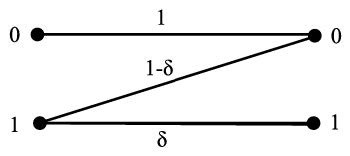
\includegraphics[height=2.5cm]{img/6-3.jpg}
  \caption{Z-Channel}
  \label{fig:z-chan}
\end{figure}
}
  \begin{solution}
  Assume that $\Pr(X=1)=\pi$, given the transition matrix $Q$, we have that $\Pr(Y=1) = \frac{\pi}{2}$, $\Pr(Y=1) = 1 - \frac{\pi}{2}$.
  \begin{equation}
    \begin{aligned}
      I(X;Y)&= H(Y) - H(Y|X) \\
      &= H(\frac{\pi}{2}) - \pi H(\frac{1}{2}) - (1-\pi)H(1) \\
      &= -\frac{\pi}{2} \log(\frac{\pi}{2}) - \left(1 - \frac{\pi}{2}\right) \log \left(1 - \frac{\pi}{2}\right) - \pi
    \end{aligned}
  \end{equation}
  Since the function is a concave function, we find its maximal value by taking the derivative.
  \begin{equation}
    \begin{aligned}
      \frac{dI(X;Y)}{d\pi} &= -\frac{1}{2} \log(\frac{\pi}{2}) - \frac{1}{2\ln 2} + \frac{1}{2\ln 2} + \left(1 - \frac{1}{2}\right) \log \left(1 - \frac{\pi}{2}\right) -1 \\
      &= \frac{1}{2} \log \frac{2-\pi}{\pi} - 1 := 0      
    \end{aligned}
  \end{equation}
  It follows that the mutual information is at its maximum when $\pi = \frac{2}{5}$. The channel capacity is $C \approx 0.32193$.
  \end{solution}
  \label{ex4}
\end{exercise}

%%%%%%%%%%%%%%%%%%%%%%%%%%%%%%%%%%%%%%%%%%
%%%%%%%%%%%%%                 %%%%%%%%%%%%
%%%%%%%%%%%%%    EXERCISE 5   %%%%%%%%%%%%
%%%%%%%%%%%%%                 %%%%%%%%%%%%
%%%%%%%%%%%%%%%%%%%%%%%%%%%%%%%%%%%%%%%%%%
\begin{exercise}[Erasures and errors in a binary channel]{Consider a channel with binary inputs that has both erasures and errors. Let the probability of error be $\epsilon$ and the probability of erasure be $\alpha,$ so the channel is follows:
  \begin{figure}[H]
    \centering
    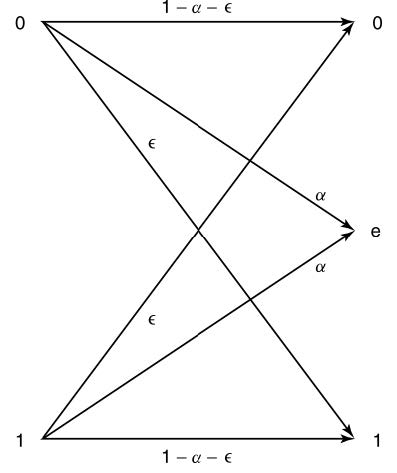
\includegraphics[height=5cm]{img/6-4.jpg}
    \caption{Erasures and Errors}
    \label{fig:err}
  \end{figure}
  Find the capacity of this channel.}
  \begin{solution}
    The transition matrix is as follows.
    \begin{table}[H]
      \begin{center}
        \begin{tabular}{c|ccc}
         \diagbox{X}{Y} & 0             & e             & 2             \\ \hline
        0 & $1-\alpha-\epsilon$ & $\alpha$ & $\epsilon$             \\
        1 & $\epsilon$            & $\alpha$ & $1-\alpha-\epsilon$
        \end{tabular}
      \end{center}
      \end{table}
      The matrix is row symmetric, we have that
      \begin{equation}
        I(X ; Y) = H(Y)-H(Y | X) = H(Y) - H(\alpha,\epsilon,1-\alpha-\epsilon)
      \end{equation}
      Furthermore, note that the distribution of $Y$ in terms of the distribution of $X$ is symmetric, i.e. 
      \begin{equation}
        H(Y) \arrowvert_{\Pr(X=0)=\pi} = H(Y) \arrowvert_{\Pr(X=0)=1 - \pi}
      \end{equation}
      and that the entropy function is a concave function. It follows that the maximal value must be obtained at $p(x) = \frac{1}{2}$ for $x = 0,1$.
      \begin{equation}
        C = H(\frac{1-\alpha}{2},\alpha,\frac{1-\alpha}{2}) - H(\alpha,\epsilon,1-\alpha-\epsilon)
      \end{equation}
  \end{solution}
  \label{ex5}
\end{exercise}

%%%%%%%%%%%%%%%%%%%%%%%%%%%%%%%%%%%%%%%%%%
%%%%%%%%%%%%%                 %%%%%%%%%%%%
%%%%%%%%%%%%%    EXERCISE 6   %%%%%%%%%%%%
%%%%%%%%%%%%%                 %%%%%%%%%%%%
%%%%%%%%%%%%%%%%%%%%%%%%%%%%%%%%%%%%%%%%%%
\begin{exercise}[Additive noise channel]{Find the channel capacity of the following discrete memoryless channel:
\begin{figure}[H]
  \centering
  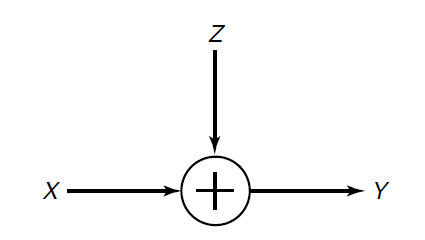
\includegraphics[height=3cm]{img/6-5.png}
  \caption{Discrete Memoryless Channel}
  \label{fig:ex6}
\end{figure}
where $\operatorname{Pr}\{Z=0\}=\operatorname{Pr}\{Z=a\}=\frac{1}{2} .$ The alphabet for $x$ is $\mathbf{X}=$ \{0,1\} . Assume that $Z$ is independent of $X .$ Observe that the channel capacity depends on the value of $a$. }
  \begin{solution}
  The condition implies that $a\neq 0$, but after the plus operation the distribution of $Y$ may vary. Hence we discuss the value of $a$ in several cases.
  \begin{enumerate}
    \item {
      $a = \pm 1$, the result of $X + a$ and $X + 0$ may overlap. We take the case of $a = 1$ as example. The transition matrix is as follows.
      \begin{table}[H]
        \begin{center}
          \begin{tabular}{c|ccc}
           \diagbox{X}{Y} & 0             & 1             & 2             \\[2mm] \hline
          0 & $\frac{1}{2}$ & $\frac{1}{2}$ & 0             \\[2mm]
          1 & 0             & $\frac{1}{2}$ & $\frac{1}{2}$
          \end{tabular}
        \end{center}
        \end{table}
        The matrix is row symmetric, assume that $\Pr(X = 0) = \pi$we have that
        \begin{equation}
          \begin{aligned}
          I(X ; Y) &=H(Y)-H(Y | X) \\
          &=H(\frac{1}{2}\pi,\frac{1}{2},\frac{1}{2}\pi)-H(\frac{1}{2}) \\
          & \leq H(\frac{1}{4},\frac{1}{4},\frac{1}{2}\pi)-H(\frac{1}{2}) = \frac{1}{2}
          \end{aligned}
        \end{equation}
        $C = \frac{1}{2}$. The maximal value is obtained at $\pi = \frac{1}{2}$.
    }
    \item{$a \neq \pm 1$. Then the output $Y$ will not overlap for different $X$. Hence $Y$ is a function of $X$. We have
    \begin{equation}
      C=\max I(X ; Y)=\max H(X) = 1
    \end{equation}
    The maximal value is obtained when $p(x) = \frac{1}{2}$ for $x=0,1$.
    }
  \end{enumerate}
  \end{solution}
  \label{ex6}
\end{exercise}

%%%%%%%%%%%%%%%%%%%%%%%%%%%%%%%%%%%%%%%%%%
%%%%%%%%%%%%%                 %%%%%%%%%%%%
%%%%%%%%%%%%%    EXERCISE 7   %%%%%%%%%%%%
%%%%%%%%%%%%%                 %%%%%%%%%%%%
%%%%%%%%%%%%%%%%%%%%%%%%%%%%%%%%%%%%%%%%%%
\begin{exercise}[Channel capacity]{Consider the discrete memoryless channel $Y=$ $X+Z(\bmod 11),$ where
  $$
  Z=\left(\begin{array}{ccc}
  1, & 2, & 3 \\
  \frac{1}{3}, & \frac{1}{3}, & \frac{1}{3}
  \end{array}\right)
  $$
  and $X \in\{0,1, \ldots, 10\} .$ Assume that $Z$ is independent of $X$.
  \begin{enumerate}
    \item Find the capacity.
    \item What is the maximizing $p^{*}(x) ?$
  \end{enumerate}}
  \begin{solution} Note that the transition matrix of this channel is
    \begin{table}[H]
      \begin{center}
        \begin{tabular}{c|cccccc}
          \diagbox{$X$}{$Y$}         & 0             & 1             & 2             & $\ldots$ & 9        & 10            \\[2mm] \hline
        0        & 0             & $\frac{1}{3}$ & $\frac{1}{3}$ & $\ldots$ & 0        & 0             \\[2mm]
        1        & 0             & 0             & $\frac{1}{3}$ & $\ldots$ & 0        & 0             \\[2mm]
        2        & 0             & 0             & 0             & $\ldots$ & 0        & 0             \\[2mm]
        $\vdots$ & $\vdots$      & $\vdots$      & $\vdots$      & $\ddots$ & $\vdots$ & $\vdots$      \\[2mm]
        9        & $\frac{1}{3}$ & $\frac{1}{3}$ & 0             & $\ldots$ & 0        & $\frac{1}{3}$ \\[2mm]
        10       & $\frac{1}{3}$ & $\frac{1}{3}$ & $\frac{1}{3}$ & $\ldots$ & 0        & 0            
        \end{tabular}
      \end{center}
    \end{table}
    Note that the matrix is both column and row symmetric. Therefore we have
    \begin{equation}
      \begin{aligned}
        I(X ; Y) &=H(Y)-H(Y | X) \\
        &=H(Y)-H(\mathbf{r}) \\
        & \leq \log |\mathcal{Y}|-H(\mathbf{r}) = \log 11 - \log 3 = \log \frac{11}{3}
        \end{aligned}
    \end{equation}
    $C = \log \frac{11}{3}$. The maximal value is obtained when $p^{*}(x) = \frac{1}{11}$ for every $x \in \{0,1, \ldots, 10\}$
  \end{solution}
  \label{ex7}
\end{exercise}

%%%%%%%%%%%%%%%%%%%%%%%%%%%%%%%%%%%%%%%%%%
%%%%%%%%%%%%%                 %%%%%%%%%%%%
%%%%%%%%%%%%%    EXERCISE 8   %%%%%%%%%%%%
%%%%%%%%%%%%%                 %%%%%%%%%%%%
%%%%%%%%%%%%%%%%%%%%%%%%%%%%%%%%%%%%%%%%%%
\begin{exercise}[Zero-error capacity]{A channel with alphabet \{0,1,2,3,4\} has transition probabilities of the form
  $$
  p(y | x)=\left\{\begin{array}{cl}
  1 / 2 & \text { if } y=x \pm 1 \bmod 5 \\
  0 & \text { otherwise }
  \end{array}\right.
  $$
  (a) Compute the capacity of this channel in bits.

  (b) The zero-error capacity of a channel is the number of bits per channel use that can be transmitted with zero probability of error. Clearly, the zero-error capacity of this pentagonal channel is at least 1 bit (transmit 0 or 1 with probability $1 / 2$ ). Find a block code that shows that the zero-error capacity is greater than 1 bit. Can you estimate the exact value of the zero-error capacity? (Hint: Consider codes of length 2 for this channel.)}
  \begin{solution}
  \begin{enumerate}
    \item {
      Note that the transition matrix is row and column symmetric. It follows that
      \begin{equation}
        \begin{aligned}
          I(X ; Y) &=H(Y)-H(Y | X) \\
          &=H(Y)-H(\frac{1}{2}) \\
          & \leq \log |\mathcal{Y}|-H(\frac{1}{2}) = \log 5 - 1 \approx1.322
          \end{aligned}
      \end{equation}
      $C = 1.322$ bits. The maximal value is obtained when $X$ and $Y$ are uniformly distributed.
    }
    \item {
      According to the hint, we try to build a 2-tuple code with the alphabet \{0,1,2,3,4\}. Note that for every input codeword $\left(X_1,X_2\right)$, there are four possibilities of output, namely $\left((X_1 \pm 1) \bmod 5 ,(X_1 \pm 1) \bmod 5\right)$, but the good news is that if we can ensure that there are no other input codewords (and their possible outputs) occupying the 4 entries, we can infer the input determintly.
      
      Figure \ref{fig:ex8} gives an example of zero-error codes, where cells identified by different colors represent a codeword. The input codewords are (0,0),(1,2),(2,4),(3,1) and (4,3). Given an output codeword, its corresponding input codeword can be determined directly from the table.
      \begin{figure}[H]
        \centering
        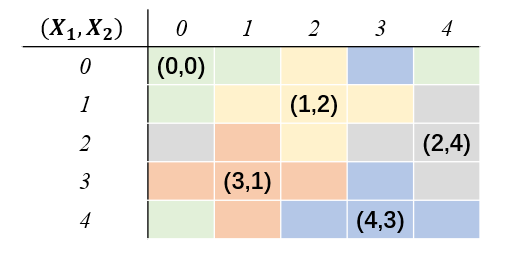
\includegraphics[]{img/6-6.png}
        \caption{A Construction of Zero-Error Codes}
        \label{fig:ex8}
      \end{figure}

      With the codes above, we can find that the number of bits per channel use is $\frac{1}{2} \log{5} > 1$.
    }
  \end{enumerate}
  \end{solution}
  \label{ex8}
\end{exercise}

\end{document}
